\begin{minipage}[t]{180mm}
\fcolorbox{black}{white}{
\begin{minipage}[b]{30mm}

\includegraphics[width=0.5\linewidth]{unflogo.pdf}
\end{minipage}
\begin{minipage}[b]{100mm}
\Huge \textbf{UNF NEWZ} \\
\Large -- Søvn og retsstavning er overvurderet! 
\end{minipage}
\begin{minipage}[b]{50mm}
\Large Onsdag 17.07.2015 \\
\normalsize Redigeret i \LaTeX\ af \\ SOM, MGS, MMN, SABH
\end{minipage}
}
\end{minipage}



\begin{minipage}[b]{0.95\linewidth}
\begin{minipage}[t]{0.47\textwidth}
\vspace{3mm}
\section*{Tanker fra et tog}
Dette skrives fra en mobil. Mobilen er en nymodens smartphone, som de så populært kaldes. Denne smartphone befinder sig i skrivende stund i et tog. Toget holder stille. Stille vil det holde i 5 minutter endnu. Men i disse 5 minutter vil toget stadigt og vedvarende befinde sig trygt på Aarhus Banegård, trygt i havn, selvom det ikke er et skib.\\

Det skrivende individ tænker ikke længe over de skrevne ord, men savner allerede MatCamp nok til at tænke længere end tekstens fremkomst, tænke på dem, der måske kommer til at læse den. De smukke og dejlige mennesker, som er mere end blot medarrangører, mere end bare UNF'ere - de er interessante mennesker, der er mange års venskab værd, som spreder glæde og smil, som forstår konceptet 'at være et godt menneske'. Det er derfor også med sørgmodig stemning, at der bliver kærtegnet for den fedtede touchscreen, for havde det blot været i går, havde det i stedet været den bærbares taster, der blev kælet for, ved at hamre løs på det nedslidte tastatur i et noget højere tempo, mens kaffekoppen hurtigt ville tømmes - men dette i selskab med folk, der ikke kan erstattes. \\
\\
Toget kører nu. Toget kørte et minut for sent. Mobilen kører forlæns. Personen, der holder den, kører baglæns. \\
\\
Det må desværre blive alt for nu. Ellers bliver den sørgmodige stakkel hurtigt køresyg - og der er endnu langt til destinationen.
\\
\\
Hav den bedste Camp - NOGENSINDE!
{\flushright\emph{Jasmin - Syltetøj aka JAM aka wannabe jyde}}

\end{minipage}
\hfill\begin{minipage}[t]{0.47\textwidth}

\vspace{1mm}
\tikzstyle{mybox} = [draw=white, fill=blue!20, very thick,
    rectangle, rounded corners, inner sep=10pt, inner ysep=20pt]
\tikzstyle{fancytitle} =[fill=red, text=white]

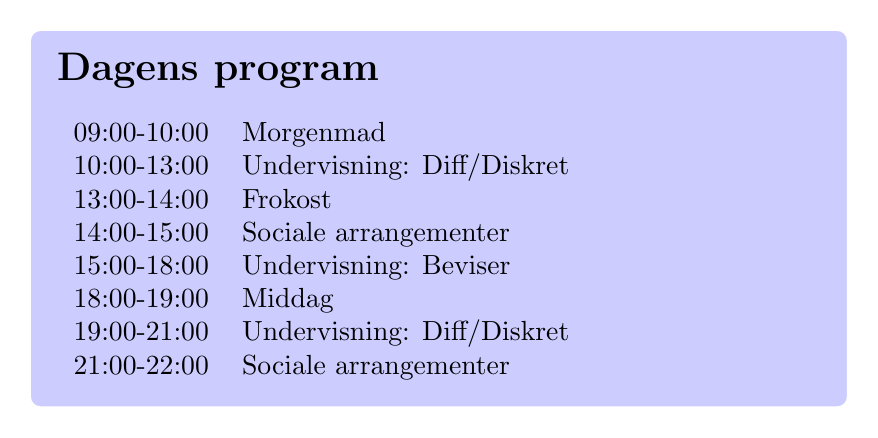
\begin{tikzpicture}
\node [mybox] (box){%
\begin{minipage}{0.80\textwidth}
\vspace{-4mm}\section*{Dagens program}
\begin{tabular}{ll}
09:00-10:00 & Morgenmad \\
10:00-13:00 & Undervisning: Diff/Diskret \\
13:00-14:00 & Frokost \\
14:00-15:00 & Sociale arrangementer \\
15:00-18:00 & Undervisning: Beviser \\
18:00-19:00 & Middag \\
19:00-21:00 & Undervisning: Diff/Diskret \\
21:00-22:00 & Sociale arrangementer
\end{tabular}
\vspace{-4mm}
\end{minipage}
};
\end{tikzpicture}%



\end{minipage}
\end{minipage}
